\section{Redshift distribution of galaxies}

In this section we look at question 1 subquestion a, 
we want to add this extra explanation bla bla, and also 
note bla bla. \\

Below shows the script for problem 3:



\begin{enumerate}[label=(\alph*)]
    \item The script for implementing the basic LU decomposition is:
    \lstinputlisting{problem3a.py}
    Giving output:
    \lstinputlisting{problem3a.txt}
    \item The script for implementing the basic LU decomposition is:
    \lstinputlisting{problem3b.py}
    \begin{figure}[h!]
    \centering
    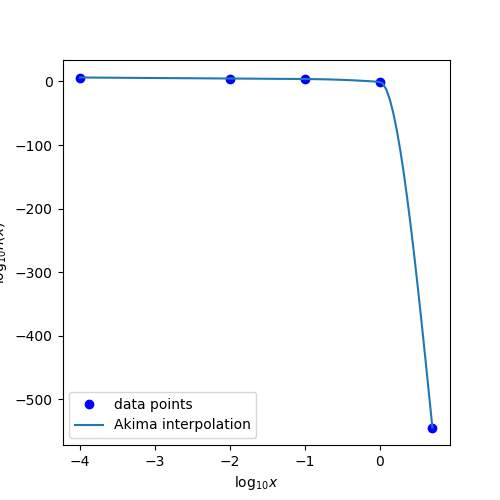
\includegraphics[width=0.9\linewidth]{./problem3.png}
    \caption{Log-log plot for n as a function of x.  Here Akima sub-spline algorithm is used for interpolation.}
    \label{fig:fig1}
    \end{figure}
    Giving output:
    \lstinputlisting{problem3b.txt}
    \lstinputlisting{problem3c.py}
    Giving output:
    \lstinputlisting{problem3c.txt}
\end{enumerate}




